%Primera clase de Producción Gráfica con Tikz.
%%%%%%%%%%%%%%%%%%%%%%%%%%%%%%%%%%%%%%%%%%%%%%
%Anotaciones:
%¿Qué es standalone?
%Nos permite ajustar el tamaño del documento
%%%%%%%%%%%%%%%%%%%%%%%%%%%%%%%%%%%%%%%%%%%%%%
\documentclass{standalone}%También se puede usar article
\usepackage{tikz}
\usetikzlibrary{babel,calc}
%\usetikzlibrary{positioning}

%\tikzset{3D/.cd,
%	x/.store in=\xx, x=0,
%	y/.store in=\yy, y=0,
%	z/.store in=\zz, z=0
%}
%\usepackage[utf8x]{inputenc}%Nos permite reconocer algunas tipografías.
%\usepackage[spanish]{babel}
%\usepackage{tikz}%%%Paquete principal
\usetikzlibrary{babel,arrows,calc}

%Permite usar flechas con dobles puntas.
\begin{document}
%hello \tikz \draw[red] (0, .5) -- (1.5, .5); mundo tikz%\\ %[->] Se define las coordenas de un punto
%hello \tikz \draw[red] (0, .5) -- (1.5pt, .5); mundo tikz%\\ %[->] 
%hello \tikz \draw[red] (0, .5) -- (1.5mm, .5); mundo tikz%\\ %[->] 
%trabaja con coordenadas cartesianas, desde la coordenada (0,.5) hasta ()
%¿Se puede graficar en coordenadas polares?
%Para usar la flecha se necesita una librer[ia de tikz.
%Qué entendemos por dinámico, no como GIF
%Ejemplo 2. Dibujar circunferencia con
%Hola \tikz \draw (0,0) circle[radius =5pt]; mundo tikz
%Puedo dibujar dentro del texto, las imágenes garantizan la ubicación.
%Ahora vamos a usar tikzpicture.
%Siempre usar ; como en C, se trabaja en coordenadas cartesianas y se asuma que la longitud por defecto es de 1cm.
%Ahora veremos el
%Dibujo de un círculo.
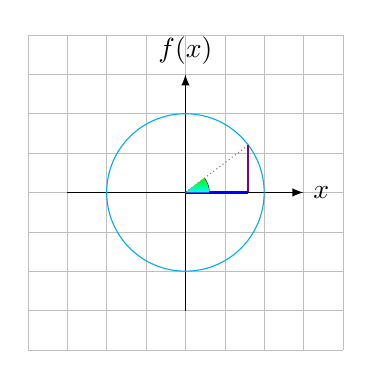
\begin{tikzpicture}
	%\clip[draw](-.1, -.1) rectangle (.5, .3); %Mapa y marco
	
	\def\t{37}
	\def\tr{(\t * pi)/180};
	\draw[gray!50, very thin, xstep = .5, ystep = .5] (-2, -2) grid (2,2);
	%\clip(-.1, -.1) rectangle (.5, .3); %Mapa y marco
	%\clip(.15, 0) circle (.5cm); %Mapa y marco, recorte y aproximaciones.
	\draw[>=latex, ->] (-1.5,0) -- (1.5, 0) node[right] {$x$};%above 
	\draw[>=latex, ->] (0, -1.5) -- (0, 1.5) node[above] {$f(x)$};% left
	
	\draw[cyan](0,0) circle[radius =1];
	%\draw (0,0) ellipse[x radius =2, y radius =1]; %Elipse de R_h=2cm y R_v=1cm.
	%\draw (0,0) rectangle (2,2);%--(3,0) --cycle
	%\draw (0,0) -- (3,0) -- %(1.5, 1.5) -- cycle;
	\draw (3mm, 0) arc[start angle = 0, end angle = \t, radius =.3];%dashed, thin, dotted,loosely
	\draw[line width =.05pt, thin, densely dotted, gray] (0, 0) -- (\t:1);%[]very thin
	%\draw (0,0) +(\t:1) -- ++(0, {sin(\t)});%Recta horizontal
	%\draw (0,0) +(\t:1) -- ++(0, -{sin(\t)});%Recta oblicua
	\draw[line width =.7pt, red!50!blue](0,0) ++(\t:1) -- ++(0, -{sin(\t)});%Recta oblicua
	\draw[line width =1pt, blue] (0,0) -- (+{cos(\t)}, 0);
	\fill[magenta] (0,0) -- (.3, 0) arc[start angle = 0, end angle = \t, radius =.3] -- cycle; %Solo se usa para regiones cerradas. cycle
	\shade[top color = green, bottom color = cyan] (0,0) -- (.3, 0) arc[start angle = 0, end angle = \t, radius =.3] -- cycle;%inner y outer de adentro hacia afuera. [ball color =cyan] como efecto de brillo.
	%Estamos enmarcando la región 
	%Se usa coordenadas relativas, fíjese 
	%Cycle se usa para dibujar caminos cerrados.
	%Calc nos usa para dibujar 
	%Se le suma a (0,0) (\t,1), con doble ++ se vuelve nuestro nuevo punto de referencia.
	%Se hace nuevo punto de referencia con ++, puedo usarlo muchas veces.
	%¿Cómo usar saltos de líneas en textos? Usando nodos como cajas de textos.
\end{tikzpicture}
%Se puede usar otro tipo de coordenadas?
%Hemos visto segmentos de líneas, arcos, coordenadas absolutas y relativas.
%Librería calc
%Tikz carga el paquete xcolor.
\end{document}
En la pregunta anterior, si hay diferencia, pues afectaría a las coordenadas del siguiente
Ahora vamos a ver colores de relleno. Usaremos clic para utilizar un resorte.
Qué es un relleno degradado.
\fill
\filldraw
\shade